\documentclass[a4paper]{article}

\usepackage{a4wide}
\usepackage{graphicx}

\author{Bram Pulles}
\title{\textbf{bTCP: basic Transmission Control Protocol}}

\begin{document}
\maketitle

\tableofcontents
\pagebreak

\section{Finite state machines}
This section describes all of the finite state machines for bTCP. In every finite state machine figure, the transitions where messages are received or send have the part being received on top and the part being send underneath. Further, a - indicates that nothing is send/received. At last, everything before the vertical bar indicates the flags which are set and everything after the bar is the content/values of the segment.

	\subsection{Connection establishment}
	The finite state machines for the establishment of a connection can be seen in figure \ref{fig: phase 1 client} and \ref{fig: phase 1 server}, for the client and server respectively. Note that we do not verify if the server received the last ACK. This is not implemented in the code and could potentially cause a failure if the ACK is not received and the client already starts to send data. However, the chance that this ACK would get lost is considerably small.
	\begin{figure}[h]
		\centering
		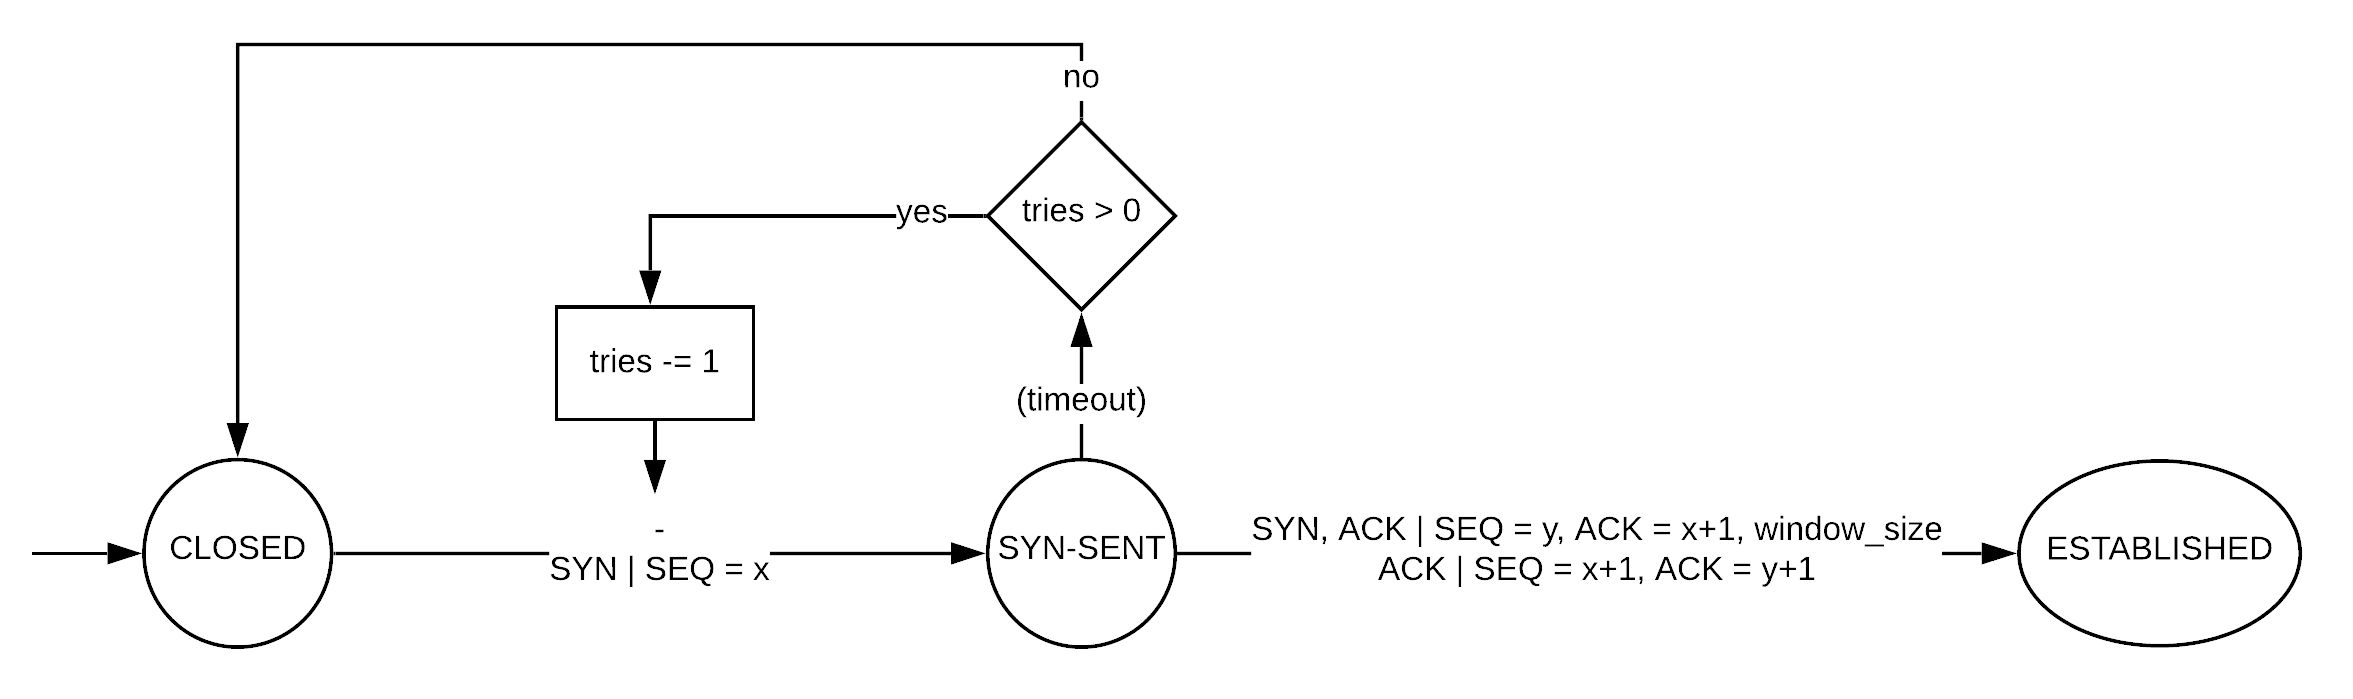
\includegraphics[width = \textwidth]{phase1_client.png}
		\caption{FSM connection establishment client.}
		\label{fig: phase 1 client}
	\end{figure}
	\begin{figure}[h]
		\centering
		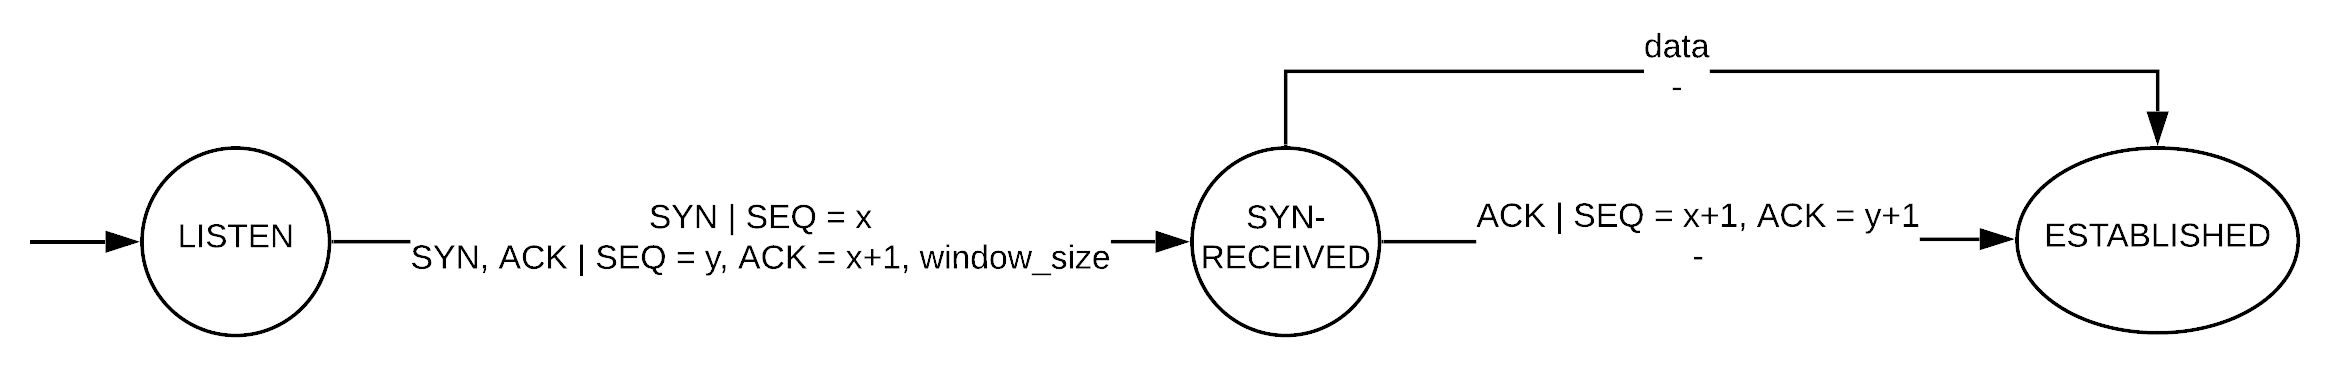
\includegraphics[width = \textwidth]{phase1_server.png}
		\caption{FSM connection establishment server.}
		\label{fig: phase 1 server}
	\end{figure}

	\subsection{Sending/receiving data}
	The finite state machines for an established connection where data is being send can be seen in figure \ref{fig: phase 2 client} and \ref{fig: phase 2 server}, for the client and the server respectively. The FSM for the server is extremely simply, since it only sends back ACKs for segments it received, that is all.
	% TODO Add finite state machine for the client.
	\begin{figure}[h]
		\centering
		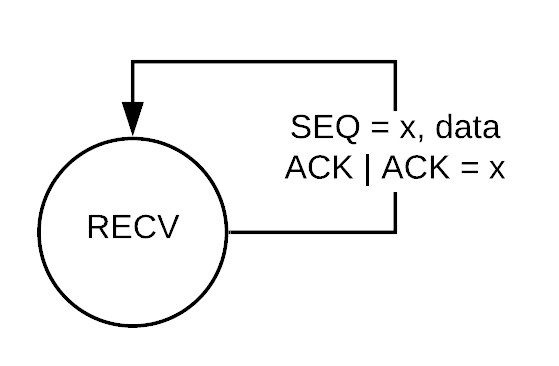
\includegraphics[width = .3\textwidth]{phase2_server.png}
		\caption{FSM receiving data server.}
		\label{fig: phase 2 server}
	\end{figure}

	\subsection{Connection termination}
	The finite state machines for the termination of a connection can be seen in figure \ref{fig: phase 3 client} and \ref{fig: phase 3 server}, for the client and server respectively. Note that the server does not verify if the ACK send is received by the client. However, since the client terminates the connection after having done a certain amount of tries (each with a timeout), it does not matter since both will close correctly anyways.
	\begin{figure}[h]
		\centering
		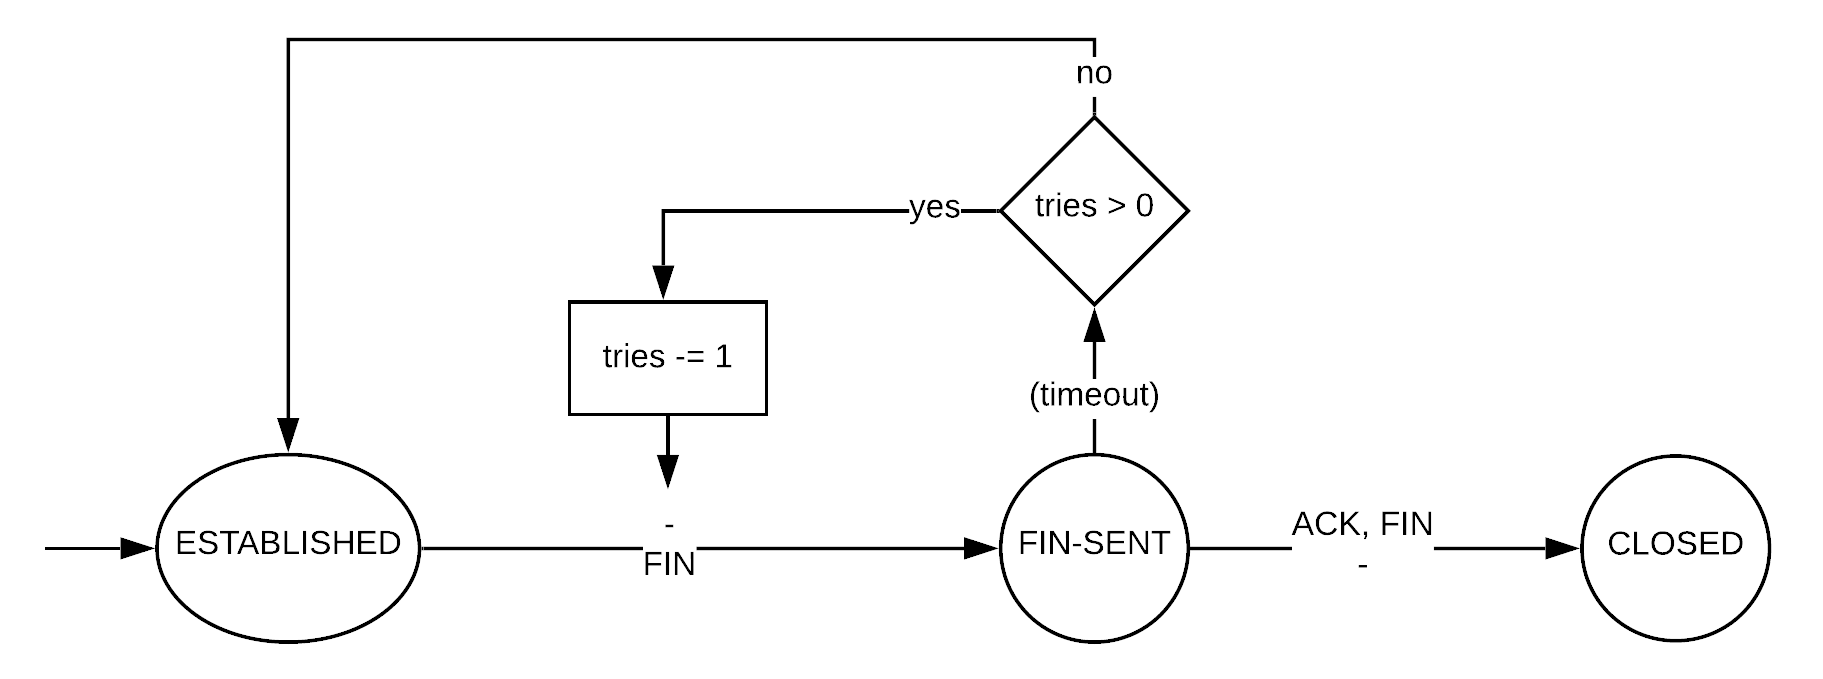
\includegraphics[width = \textwidth]{phase3_client.png}
		\caption{FSM connection termination client.}
		\label{fig: phase 3 client}
	\end{figure}
	\begin{figure}[h]
		\centering
		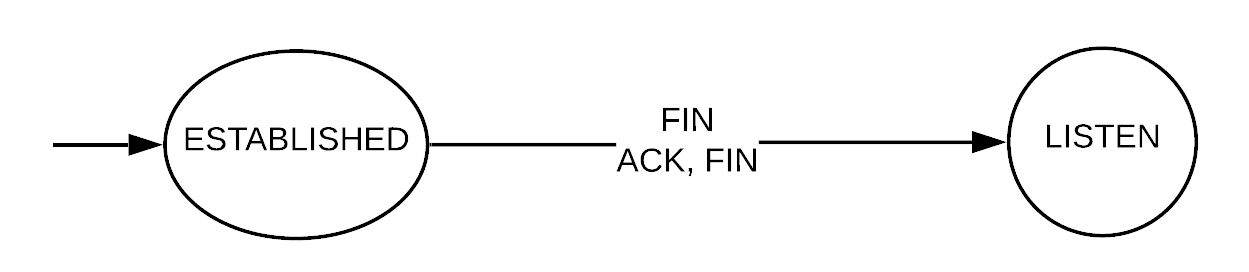
\includegraphics[width = .7\textwidth]{phase3_server.png}
		\caption{FSM connection termination server.}
		\label{fig: phase 3 server}
	\end{figure}

\section{Reliability}

\section{Flow control}

\section{File transfer}

\section{Implementation}
This section describes some design choices on the implementation level.

	\subsection{bTCP socket interface}
	The description of the bTCP protocol in the assignment tells us that we only need to have traffic being send from the client to the server. The server will only send ACKs back to the client for receiving its data. This means that we only need to think about the receiving window of the server. It also means that only the client needs to keep a timer in order to determine when to resend a packet.

	The template provided for this project does not account for this and gives a timeout and window size parameter to both the client and the server even though they both only need one. I refractored the bTCP socket interface so it does not need to be a class anymore containing these variables. This makes it easier to test the individual functions as well as providing a cleaner code base, since unnecessary variables are removed from both the client and the server.


\end{document}
